
\chapter{Introducción}

% todo: AGREGAR FONTANELLA Y VIDAL DE BATTINI
% RESCRIBIR

El uso de la lengua siempre ha caracterizado a las personas que la utilizan. La forma en que nos comunicamos no sólo posee la información del mensaje a trasmitir, sino que también posee características del hablante. Estudiar estas características del habla nos permite conocer mejor la cultura de las personas. Nos permite identificar a los hablantes para saber el lugar donde pertenecen.

Identificar y extraer características del habla es una tarea muy difícil de realizar. No solo se debe obtener muestras muy variadas de muchos hablantes en distintas regiones, sino que también hay que prestarle importante atención a su edad, su sexo, su situación económica, etc. Realizar un estudio de estas características es muy complejo y, por sobre todo, costoso. Además de estudiar cada grupo se debe utilizar muchos recursos: por ejemplo, se deben utilizar soporte para grabar en buena calidad las muestras, se debe realizar varios viajes para buscar los diferentes hablantes, se debe analizar cada uno de los audios de manera individual, entre otras cosas. 

\begin{figure}[h!]
	\centering
    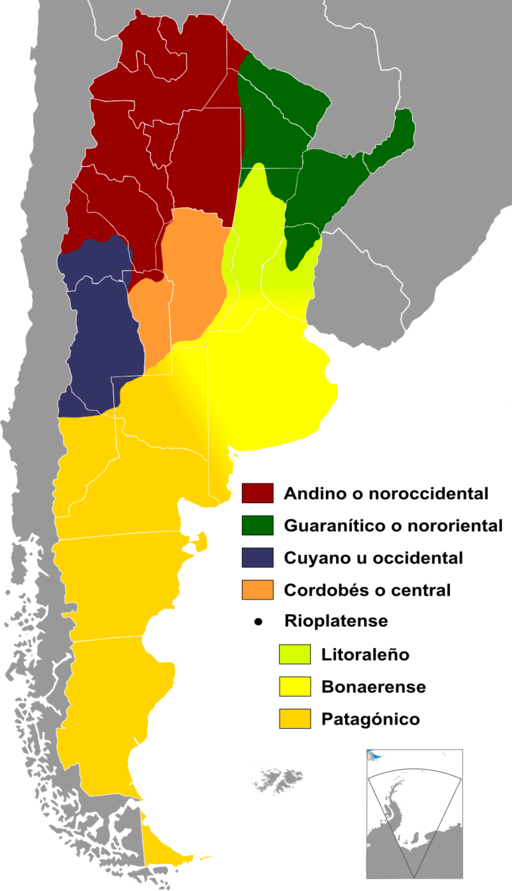
\includegraphics[width=0.5\textwidth]{Dialectos_del_idioma_espanol_en_Argentina} 
    \caption{Dialectos del idioma español en Argentina}
    \label{fig11}
\end{figure}

La motivación de esta tesis es realizar un sistema que pueda facilitar estos problemas. Vamos a enfrentar cada uno de ellos e intentar resolverlos de forma computacional. De los problemas descriptos el principal radica en obtener cada grabación. Si los grupos se encuentran muy alejados esto puede ser muy costoso por los viajes. También estas grabaciones deben ser de calidad aceptable como para realizar el estudio en cuestión. Se podría utilizar el teléfono para algunos experimentos pero hay que tener en cuenta que posee calidad muy baja. De hecho, se utiliza en algunos experimentos donde esta característica no es un inconveniente. 

El sistema desarrollado utiliza Internet como herramienta para obtener muestras. De esta forma, se puede realizar varias grabaciones sin necesidad de viajar a cada lugar. Es cierto que no todos los lugares poseen acceso a Internet y, si se realizara un experimento de estas características en lugares carenciados que no posean una conexión, este sistema no sería útil. De cualquier forma, pensamos que su utilización soluciona muchos inconvenientes. Otra ventaja radica en que se puede manejar la calidad de la grabación. Utilizando distintas tecnologías a través de esta red se puede configurar la calidad para que sea lo más precisa posible para el experimento. Vamos a realizar un sistema para mejorar este proceso y diseñaremos un experimento para corroborar las ventajas y desventajas del mismo.

El experimento que tomamos como caso particular es las diferencias en el habla entre Córdoba y Buenos Aires. Estos dos grupos se encuentran uno en la zona central de nuestro país y el otro cerca del Río de la Plata, como se puede observar en la Figura \ref{fig11}. En la literatura existen estudios que explican estas diferencias, por ejemplo \textit{El español en la Argentina} \cite{Fontanella2000} de Beatriz Fontanella de Weinberg y \textit{Español en la Argentina} \cite{Vidal1964} de Elena Vidal de Battini. 

Fontanella de Weinberg recompila varios trabajos de colegas que analizan el español de cada región de Argentina. Cada región se describe en un capítulo distinto y entre ellas se encuentra uno para Buenos Aires y otro para Córdoba. En la descripción de estos capítulos las diferencias hacen hincapié en los sonidos más suaves y cortos de la /r/ y la /i/ y en la aspiración de la /s/. También describe el estiramiento de la sílaba anterior a la acentuada en cada palabra como distintivo del acento. Por su parte, Vidal de Battini analiza región por región el uso de los fonemas importantes. Destaca la diferencia entre las dos regiones de la /r/, /s/ y de la /ll/. También referencia a la pronunciación de la /s/.
%pagina 85 Fontanella 

Extrayendo el análisis de estos libros pude definir las reglas que describen a cada grupo. Las reglas son: 

\begin{itemize}

\item \textbf{Regla 1: Los hablantes de Córdoba estiran la sílaba anterior a la acentuada mientras los de Buenos Aires no realizan esto.} Cada palabra posee una sílaba con su acento primario. Para cumplir esta regla se debe estirar la sílaba anterior a esta. Si la sílaba acentuada es la primera de la palabra, entonces no se estira. Ejemplo: `Espectacular' posee su sílaba acentuada en `-lar'. La sílaba anterior, o sea `-cu-' se alarga solamente para hablantes de Córdoba. 

\item \textbf{Regla 2: Los hablantes de Córdoba aspiran y elisionan la /s/ al finalizar una palabra. Esto no sucede para Buenos Aires.} Para las palabras terminadas en /s/ se acorta su duración en el hablante de Córdoba. Ejemplo: `Pájaros' posee el fonema /s/ al final. Utilizando la dialéctica de Córdoba, la /s/ final sería mas suave que una de Buenos Aires. 

\item \textbf{Regla 3: Para hablantes de Córdoba, la /s/ antes de la /c/ o /t/ suenan más suaves que para hablantes de Buenos Aires.} La sílaba /s/, que precede a /c/ o /t/, suena más suave en cordobeces que en porteños. Ejemplo: `Mosca' en la variante de Córdoba posee una sílaba más suave en el fonema /s/ que en Buenos Aires. 

\item \textbf{Regla 4: La `c' antes de la `t' se pronuncia con menor frecuencia para hablantes de Córdoba que para hablantes de Buenos Aires.} La sílaba /c/, que precede a /t/, no se debe pronunciar. Ejemplo: `Doctor' no debe sonar el fonema /c/.

\item \textbf{Regla 5: Para hablantes cordobeces la `y’ y `ll’ se pasa a `i’. No sucede esto para Buenos Aires.} Palabras con el fonema /y/ o /ll/ se pronuncian /i/. Ejemplo: `lluvia' se debe pronunciar utilizando el fonema /i/ 

\item \textbf{Regla 6: En hablantes cordobeces la /r/ no debe vibrar mientras que en Buenos Aires pasa lo contrario.} Palabras con el fonema /r/ deben ser suaves y no vibrar. Ejemplo: `Espárrago' debe ser suave en comparación de Buenos Aires. 

\end{itemize}

Cabe destacar que estas reglas se producen en el habla espontánea. Tienden a no surgir en el habla leída. Algunas pueden agudizarse si se encuentran en lugares económicamente más vulnerables, pero en cualquier ambiente se cumple.

En el próximo capítulo describiremos el diseño del experimento. Este tiene como objetivo reconocer las diferencias planteadas con las reglas mediante la grabación de frases. Estas frases fueron grabadas tanto por hablantes de Córdoba como por de Buenos Aires. También describiremos cuales frases utilizamos y el medio empleado para grabar.
